\documentclass{subfiles}

\begin{document}

    \subsection{Degrees of freedom}
        The degrees of freedom of a system are the number of independent variables needed to describe the system fully.

        \subsubsection*{Translation, rotation, vibration}
        Single atoms only have three \textit{translational} degrees of freedom, which are their x-,y-, and z-coordinates. More complex molecules may have different states depending on their rotation, making for up to three additional \textit{rotational} degrees of freedom. For example, $O_2$ has two rotational degrees of freedom, since its symmetrical along the axis connecting the atoms.Lastly, a molecule can also vibrate. Here, the \textit{vibrational} degrees of freedom are double the number of eigen-vibrationmodes. The fact that each mode is counted twice makes for a more convenient mathematical treatment of thermodynamic equations.\\

        \noindent Due to quantummechanical effects, not every degree of freedom may be available to a system with a given energy. Hence the number of \textit{effective} degrees of freedom $f_{eff}$ is smaller than the actual number $f$ \cite[p.75-76]{heintze}.\\

        \noindent In statistical mechanics it is shown, that the inner energy $U$ of one mole is connected to the degrees of freedom as follows:
        \begin{align*}
            U=\frac{1}{2}\cdot f\cdot N_A\cdot kT=\frac{1}{2}\cdot(f_{trans}+f_{rot}+f_{vibr})\cdot N_A\cdot kT.
        \end{align*}
        At constant volume the change heat $\Delta Q$ is equal to $\Delta U$ and thus the above equation gives
        \begin{align*}
            \Delta Q=\frac{1}{2}\cdot f\cdot N_Ak\cdot\Delta T=\frac{f\cdot R}{2}\cdot\Delta T\implies C_V=\frac{1}{2}\cdot f\cdot R
        \end{align*}
        for the thermal capacity $C_V$. At constant pressure, the ideal gas law gives $\Delta Q=\Delta U+p\cdot\Delta V$ and furthermore
        \begin{align*}
            \Delta Q=(C_V+R)\cdot\Delta T\implies C_p=C_V+R.
        \end{align*}
        Using the relation $\kappa=C_p/C_V$ to the isentropic exponent it follows
        \begin{align*}
            \kappa=\frac{f+2}{f},
        \end{align*}
        which can be used to determine the effective degrees of freedom of a given substance \cite[p.296-297]{demtroeder1.9}.

        \subsubsection*{Standing waves and resonance}
        Let $\psi(t,x)=A\cos(\omega t+kx)$ be a one-dimensional wave. If $\psi$ hits a reflective surface, another wave $\psi'(t,x)=A\cos(\omega t-kx+\varphi)$ of opposite direction of progragation is emitted. Both waves intefere to a singular disturbance
        \begin{align*}
            \Psi(t,x)=2A\cdot\cos(kx-\frac{\varphi}{2})\cdot\cos(kx+\frac{\varphi}{2}),
        \end{align*}
        which has fixed spots of either zero or maximal amplitude, respectively called \textit{nodes} and \textit{antinodes}. For that reason, we say $\Psi$ is a \textit{standing wave}. The phase difference $\phi$ is dependant on the given boundary conditions \cite[p.405]{demtroeder1.9}.\\

        \subsubsection*{Forced oscillations}
            Systems of vibrations can be driven by an external force, resulting in two types of oscillation: one that is typical for the system if no driving force is present, and one directly maintained by the same force. For example, if we have a harmonic oscillator and a driving force $F$, we can describe the system with
            \begin{align*}
                \ddot x(t)+\gamma\cdot\dot x(t)+\omega_0^2\cdot x(t)=F(t)
            \end{align*}
            The two types of oscillations here can be identiftied with the homogenous and inhomogenous solution to the differential equation.\\

            \noindent If damping is present, the homogenous vibration may vanish as time goes on, only leaving the inhomogenous type (if $F$ is also periodical). Due to the inertia of all mechanical systems, that second oscillations has a phase difference compared to the oscilating force $F$. For certain \textit{resonance frequencie}, this leads to the system-vibrations of much higher amplitudes than the one of $F$. Figure presents a qualitative relationship of the driving frequency $\omega$ and the amplitde of the system \cite[374-377]{demtroeder1.9}.

            \begin{figure}[H]
                \centering
                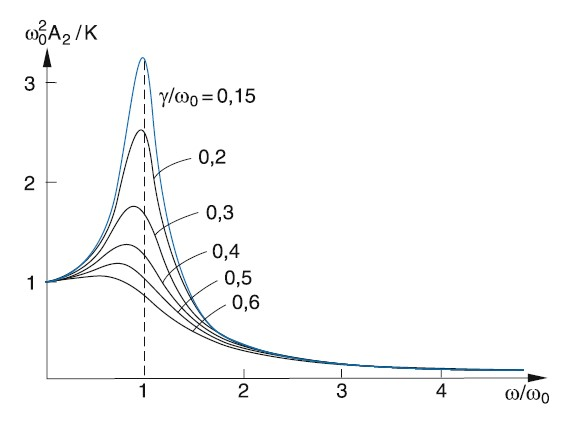
\includegraphics[width=8cm]{Bilddateien/Grundlagen/Resonanzkurve.jpg}
                \caption{resonance of a simple system for different damping coefficients $\gamma$ - for $\gamma=0$ the system can approach an unbonded amplitde, called \textit{resonance disaster}}
            \end{figure}
            
            In the case of standing waves, one may think of waves being continouesly fed into a tube of length $L$. There, they reflect of off the tubes walls, creating a standing wave. For sound waves it turns out, the resonance frequencies of that system are these, for which the wavelength fulfills the following property:
            \begin{align}
                n\cdot\frac{\lambda}{2}=L\qquad n\in\N
                \label{eq:ResonanceWavelengths}
            \end{align}
            This just means that at both ends of the tube the standing tube has either a node or antinode. Waves of frequencies that do not uphold this constraint quickly dissipate.\\

            \noindent Using \eqref{eq:ResonanceWavelengths} and $c=f\cdot\lambda$, we obtain the for velocity of sound
            \begin{align*}
                c=\frac{2\cdot f\cdot L}{n}\qquad n\in\N.
            \end{align*} 

    \subsection{Sound}
        Sound waves are longitunal pressure waves, meaning they carry changes in pressure in a direction parallel to the progragation of the wave. For high enough frequencies, this local change in pressure also causes a change in temperature.

        \subsubsection*{Velocity of sound}
            If the exchange of Temperature is slow compared to the frequency of the waves, it is reasonable to assume neglible exchange of heat. We thus have adiabatic conditions and $pV^\kappa=const.$ In these circumstances, the velocity of sound is given as 
            \begin{align*}
                c_{0}=\sqrt{\frac{p}{\rho}\cdot\kappa}
            \end{align*}

        \subsubsection*{Kirchhoff correction}
            For standing waves inside of narrow tubes, the thermal conductivity does lead to an significant exchange on heat despite high frequencies $f$. To account for this, we can use the \textit{Kirchhoff-correction}
            \begin{align*}
                c=c_0\cdot\nbra{1-\frac{a}{2r\cdot\sqrt{\pi\cdot f}}},
            \end{align*}
            where $r$ is the Radius of the tube and $a$ is the Kirchhoff constant.


% degrees of freedom: translation, rotation vibration
% standing waves + resonance condition in resonance tube
% forced oscillations
% velocity of sound in matter, including Kirchhoff correction
% experimental principle: determination of isentropic exponent: measurement according to Rüchhardt and Flammersfeld, measurement according to Clément and Desormes

\end{document}